\begin{frame}{going faster}
    \begin{itemize}
    \item so far: send one message, wait for acknowledgment
    \vspace{.5cm}
    \item very slow!
    \item instead, can send a bunch of parts and get them acknowledged together
    % \item need to do \textit{congestion control} to avoid overloading network
    \end{itemize}
\end{frame}

\usetikzlibrary{arrows.meta,decorations.pathreplacing,shapes.misc}

\begin{frame}{transmission window (ex: size 4)}
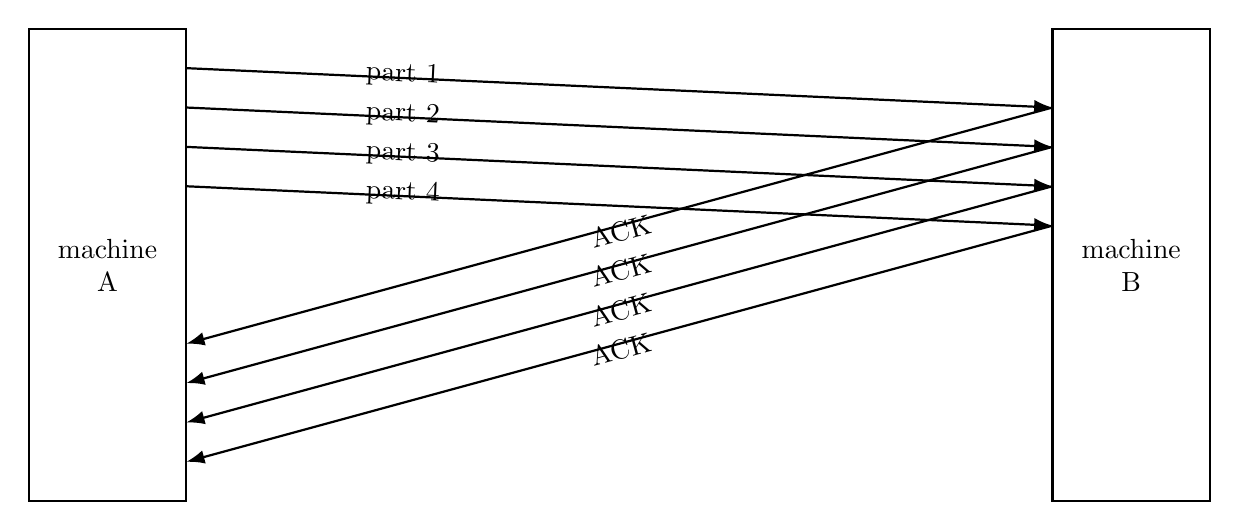
\begin{tikzpicture}
\tikzset{
    box/.style={thick},
    message/.style={draw,thick,-Latex},
    failure/.style={draw,ultra thick,red,cross out,minimum width=1cm,minimum height=1cm},
}
\begin{scope}
\draw[box] (0, 0) rectangle ++(2, -6)
    node[midway,align=center] {machine\\A};
\draw[box] (13, 0) rectangle ++(2, -6)
    node[midway,align=center] {machine\\B};
\draw[message] (2, -0.5) -- (13, -1.0) node[pos=0.25, above=-7pt, sloped] {part 1};
\draw[message] (2, -1.0) -- (13, -1.5) node[pos=0.25, above=-7pt, sloped] {part 2};
\draw[message] (2, -1.5) -- (13, -2.0) node[pos=0.25, above=-7pt, sloped] {part 3};
\draw[message] (2, -2.0) -- (13, -2.5) node[pos=0.25, above=-7pt, sloped] {part 4};
\draw[message] (13, -1.0) -- (2, -4.0) node[pos=0.5, sloped, below=-5pt] {ACK};
\draw[message] (13, -1.5) -- (2, -4.5) node[pos=0.5, sloped, below=-5pt] {ACK};
\draw[message] (13, -2.0) -- (2, -5.0) node[pos=0.5, sloped, below=-5pt] {ACK};
\draw[message] (13, -2.5) -- (2, -5.5) node[pos=0.5, sloped, below=-5pt] {ACK};
\end{scope}
\end{tikzpicture}
Send a \textit{window} of parts speculatively, then wait for ACKs.
\end{frame}
